%\documentclass[review]{elsarticle}
\documentclass[authoryear]{elsarticle}

\usepackage{lineno,hyperref}
\modulolinenumbers[5]

\usepackage{todonotes}

\journal{Journal of \LaTeX\ Templates}
%%%%%%%%%%%%%%%%%%%%%%%
% Useful Websites:
%https://www.elsevier.com/journals/atmospheric-environment/1352-2310/guide-for-authors
% https://www.elsevier.com/authors/author-schemas/latex-instructions

%%%%%%%%%%%%%%%%%%%%%%%
%% Elsevier bibliography styles
%%%%%%%%%%%%%%%%%%%%%%%
%% To change the style, put a % in front of the second line of the current style and
%% remove the % from the second line of the style you would like to use.
%%%%%%%%%%%%%%%%%%%%%%%

%% Numbered
%\bibliographystyle{model1-num-names}

%% Numbered without titles
%\bibliographystyle{model1a-num-names}

%% Harvard
%\bibliographystyle{model2-names.bst}\biboptions{authoryear}

%% Vancouver numbered
%\usepackage{numcompress}\bibliographystyle{model3-num-names}

%% Vancouver name/year
%\usepackage{numcompress}\bibliographystyle{model4-names}\biboptions{authoryear}

%% APA style
%\bibliographystyle{model5-names}\biboptions{authoryear}

%% AMA style
%\usepackage{numcompress}\bibliographystyle{model6-num-names}

%% `Elsevier LaTeX' style
%\bibliographystyle{elsarticle-num}
\bibliographystyle{elsarticle-harv}
%%%%%%%%%%%%%%%%%%%%%%%

\begin{document}

\begin{frontmatter}

%\title{Elsevier \LaTeX\ template\tnoteref{mytitlenote}}
%\title{Daily PM\textsubscript{2.5} exposure estimates by ZIP code in 11 western states differentiated by total, wildfire, and prescribed fire, 2008-2014}%\tnoteref{mytitlenote}}
\title{Daily PM\textsubscript{2.5} concentration estimates by ZIP code in 11 western states differentiated by total, wildfire, and prescribed fire, 2008-2014}%\tnoteref{mytitlenote}}
%\tnotetext[mytitlenote]{Fully documented templates are available in the elsarticle package on \href{http://www.ctan.org/tex-archive/macros/latex/contrib/elsarticle}{CTAN}.}

%% Group authors per affiliation:
%\author{Elsevier\fnref{myfootnote}}
%\author{C.E. Reid\fnref{CUfootnote},
%C.E. Reid\textsuperscript{1}, %,2\Yinyang},
%M.M. Maestas\textsuperscript{2}, 
%Ellen Considine\textsuperscript{1}, 
%N.H.F. French\fnref{MTRIfootnote}%\textsuperscript{3}, %,3\textcurrency},
%M. Billmire\textsuperscript{3}, 
%M. Jerrett\textsuperscript{4}}
%\address{Radarweg 29, Amsterdam}
%\fntext[CUfootnote]{Since 1880.}
%\fntext[MTRIfootnote]{MTRI}

%% or include affiliations in footnotes:
\author[mymainaddress]{C.E. Reid\corref{mycorrespondingauthor}}
\cortext[mycorrespondingauthor]{Corresponding author}
\ead[url]{https://www.colorado.edu/geography/colleen-reid-0}

%\author[mymainaddress,mysecondaryaddress]{Elsevier Inc}
%\ead[url]{www.elsevier.com}

\author[mysecondaryaddress]{M.M. Maestas}
%\ead[url]{www.elsevier.com}

\author[mysecondaryaddress]{G. Li}

\author[mysecondaryaddress]{E. Considine}

\author[mythirdaddress]{N.H.F. French}

\author[mythirdaddress]{M. Billmire}

\author[myfourthaddress]{M. Jerrett}

%\author[mysecondaryaddress]{Global Customer Service\corref{mycorrespondingauthor}}
%\cortext[mycorrespondingauthor]{Corresponding author}
%\ead{support@elsevier.com}

\address[mymainaddress]{Department of Geography, Guggenheim 110, 260 UCB, Boulder, Colorado 80309}%-0260, USA}
\address[mysecondaryaddress]{4001 Discovery Dr., SEEC Building Suite S348, UCB 611, Boulder, CO 80303}
\address[mythirdaddress]{Michigan Tech Research Institute, Michigan Technological University, 3600 Green Court, Suite 100, Ann Arbor, MI 48105}
\address[myfourthaddress]{UCLA Fielding School of Public Health, 650 Charles E. Young Drive South, 56-070B CHS, Los Angeles, CA 90095}

\begin{abstract} %[(about 8-10 sentences, no more than 12 sentences), about 262 words]
%[1-2 sentence indicating the problem/knowledge gap in broad terms] 
Differential risks to public health posed by air pollution from wildfires and prescribed fires are poorly understood, and a necessary pre-requisite to addressing this issue is a method to assess exposure to PM\textsubscript{2.5} differentiated among wildfire, prescribed fire, and other sources.
% [optional 1-sentence stearing toward possible sollution, i.e., machine learning]
%[1 sentence saying what we did] 
We developed a machine learning model to use earth observations to create multi-year spatiotemporal daily fine particulate matter (PM\textsubscript{2.5}) estimates attributed to prescribed fires and wildfires for 11 western states during 2008-2014.
% [2 sentences providing a little detail on what we did] 
The training data are PM\textsubscript{2.5} observations from the Environmental Protection Agency's database [check name of database], field campaigns, and monitors deployed near fires by the US Forest Service and others, and the predictor variables include MODIS and GOES aerosol optical depth (AOD), MODIS fire products, MODIS snow cover, Landsat land cover, and other Earth observations. 
To estimate the fraction of PM\textsubscript{2.5} due to each fire type, we used source-apportioned PM\textsubscript{2.5} output from the Comprehensive Air Quality Model with Extensions (CAMx). 
% [1-2 sentence describing technical/statistical method]:
[1-2 sentences to discuss machine learning method, e.g., discuss random forest, cross validation, etc.]
% [3 sentences describing results] 
[3 sentences describing results] 
% [1 sentence describing how this work is applicable/relevant in a broader context or describing need for further research]
[1 sentence describing how this work is applicable/relevant in a broader context or describing need for further research]
\end{abstract}

\begin{keyword}
wildfire \sep prescribed fire \sep PM\textsubscript{2.5} \sep spatiotemporal exposure \sep smoke
\end{keyword}
\end{frontmatter}

\linenumbers
\section{Introduction}
% % Introduction paragraph 1: set up problem >> introduce problem/gap in knowledge and motivation and give overall context
%[1 definitive sentence about something we know about the problem]
The increase in frequency and severity of landscape fires occurring in the western US \citep{Dennison2014,Steel2014} and the decrease in other sources of air pollution \citep{EPAPM25Trends2017} mean that smoke from landscape fires will be an increasingly large fraction of total air pollution.
%[1 sentence pointing out what we still don't know about the topic, (that will be answered by this paper)]
The increase in wildfires has prompted increasing pressure to engage in more prescribed burning \citep{Stephens2005}, and the public's exposure to either wildfire smoke or prescribed fire smoke are still not fully understood.
%[4 sentences providing background knowledge]



Complete fire suppression is not feasible as fire is an integral part of many ecosystems, yet many fires are suppressed to protect human populations, property and infrastructure, which can lead to a build-up of fuels that contribute to the increased intensity of wildfires in the western US \citep{Bowman2009,Schoennagel2017}.

Prescribed fires are used as a management tool to decrease fuel loads and risk of large uncontrolled wildfires while allowing for the ecological benefits of fire \citep{Schoennagel2017}. 

Previous research indicates that prescribed fires impact air quality \todo{Add citations} less than wildfires on a per-fire basis.  
Increasingly, researchers are statistically blending information from remotely-sensed Earth observations, atmospheric models, and air quality monitoring data to obtain improved spatiotemporal air pollution exposure surfaces for health studies, e.g., [citations]. \todo{Add citations}
%[1 sentence pointing out where there hasn't been enough research done]
To our knowledge, previous studies have not considered if air pollution from prescribed fires and wildfires pose differential risks to public health, and such a study would require a method for estimating differential exposures from these two sources of smoke. \todo{Check the review paper citations again, one mentions prescribed fires}
%[1 sentence citing several papers with short descriptions of what has been done in this area of research]
[1 sentence citing several papers with short descriptions of what has been done in this area of research]
%[1 sentence saying what additional studies need to accomplish]
[1 sentence saying what additional studies need to accomplish]

% Introduction paragraph 2: mechanisms - steering toward tools we'll be using - brief review of other methods that have been tried/progress, and why this isn't the final word
%[3 sentences about proposed mechanism/methods citing several papers] (3-6 sentences)
Increasingly, in the wildfire-health literature, researchers are `blending' satellite aerosol optical depth (AOD) data and air quality models together to estimate air quality exposures in locations far from monitoring sites, (e.g., \citealt{Reid2016EnvRes,Reid2015,vanDonkelaar2011,Gan2017}) as these two data sources have different strengths and weaknesses but merged together can better estimate exposures. 
Satellite AOD data has good spatial coverage, but is a measurement with of the full atmospheric column rather than at ground level. Ground-level PM\textsubscript{2.5} estimates can be extracted from air quality models, but there are uncertainties inherent in the models.
Blending these data sources over large geographic areas and long periods of time, including many fires in different locations, can provide the statistical power needed to detect if there are differential health impacts from smoke from prescribed fires and unplanned wildfires.
%[1 sentence about why the previous work is not the end of the story on this topic]
\todo{Check if true}Previous machine learning studies to estimate pollution have not considered wildfires, no [few?] studies estimating surface PM\textsubscript{2.5} have done source attribution between wildfire smoke and prescribed fire smoke.

% Introduction paragraph 3: background knowledge - elaborate about the gap in knowledge / what has been tried before, and why that is not the final word (bigger picture than next paragraph) (5-8 sentences)
Knowledge about the health impacts associated with fine particulate matter (PM\textsubscript{2.5}) from fires is important for air quality managers and  public health departments, particularly in western US states where fire can often cause public health and air quality emergencies. 
Air quality is managed at the state and local levels to conform to air quality standards set by state and federal policy.
Decisions about when to set prescribed fires involve air quality management agencies for states, tribal, and sometimes local areas in order to mitigate impacts that are both regulated and of concern for public health. 
State and local land management agencies are tasked with writing smoke management plans whenever they put fire on the ground \citep{SmokeManagement2001}. % not sure if this sentence should stay
Smoke plans involve planning burns that produce minimal smoke with maximum ecological benefit and fit within specific land management plans that consider the benefits of fire while minimizing risks related to both fire and smoke. % not sure if this sentence should stay
When projected emission levels are lower than the air quality standard for fine particulate matter (PM\textsubscript{2.5}), it is assumed that there are no health impacts, however, it is possible that health impacts could occur at that level or lower, and sometimes air pollution levels from prescribed fires reach levels higher than smoke planning tools predict.
%[1 sentence indicating the limit in knowledge]
Prescribed fires often occur in more rural areas, thus large datasets over broad geographic areas for many years are needed for statistical power, and studies cannot rely solely on monitoring data for air pollution exposure estimation as these monitors are often far from fire-impacted areas.
%[1 sentence indicating what information/knowledge would be helpful and how]
Better understanding of health impacts associated with exposure to smoke from wildfires and prescribed fires could allow better planning for future prescribed burning and targeted mitigation strategies in the face of unplanned wildfire events.

% Introduction paragraph 4: setting up this project -  Overview of what we're doing in paper (5-7 sentences)
%[1 sentence stating the hypothesis]
In this paper, we estimate total PM\textsubscript{2.5} per day attributed to all sources, and then we estimate the proportion attributed specifically to wildfires and prescribed fires to better understand the exposure of the public to air pollution from wildfires and prescribed fires as a prerequisite for future studies to examine the impacts of smoke exposure from both prescribed fires and wildfires on health.
%[1 sentence about what we did to test the hypothesis]
To accomplish this, we create a multi-year daily spatiotemporal total PM\textsubscript{2.5} exposure surface for an 11-state area in the western US for the years 2008-2014, model the transport of air pollutant emissions from each fire type (wildfire and prescribed fire), daily for the study area, and calculate daily estimates of wildfire-attributed and prescribed fire-attributed PM\textsubscript{2.5} for all ZIP codes in the study area for all 7 years.
%[1 sentence giving context, e.g., describe geographic region]
To understand if there are differential health impacts of smoke from prescribed fires and wildfires on population health, a very large dataset needs to be created and analyzed, so in this paper, we
create estimates of PM\textsubscript{2.5} source-apportioned to each fire type for a 7-year period (2008-2014) over an 11-state region of the western US (see Figure \ref{fig:Map11States}). 
%[2 sentences stating what previous studies on the topic found]
[2 sentences stating what previous studies on the topic found]
%[1 sentence indicating the gap in knowledge that remains]
Air quality managers and public health professionals in the western US want empirical evidence of the health impacts associated with prescribed fires to inform their smoke management plans and public health interventions and messaging. 
%[1 sentence describing what we did that addressed the gap in knowledge]
The objective of this paper is to use machine learning to blend MODIS and GOES aerosol optical depth (AOD), MODIS fire products, MODIS snow cover, Landsat land cover, and other Earth observations with source-apportioned fine particulate matter (PM\textsubscript{2.5}) estimates from an air quality model to create multi-year spatiotemporal PM\textsubscript{2.5} estimates attributed to prescribed fires and wildfires for 11 western states from 2008-2014.

\section{Materials and Methods}

%The author names and affiliations could be formatted in two ways:
%\begin{enumerate}[(1)]
%\item Group the authors per affiliation.
%\item Use footnotes to indicate the affiliations.
%\end{enumerate}
%See the front matter of this document for examples. You are recommended to conform your choice to the journal you are submitting to.

\paragraph{Setting} [11 western US states, 2008-2014]

[1 short paragraph]

\begin{figure}%[H] % start figure float, this method seems to have fewer options for location specifier, H, t, c, and b should work
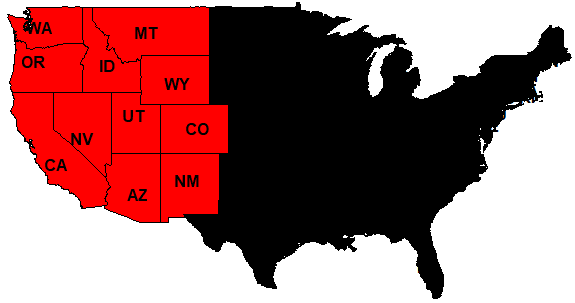
\includegraphics[width=1\textwidth]{WesternStatesNoTitleCropped.png} %
\caption{\label{fig:Map11States}Map of 11-state study area.} % The text after \label{} is what shows up as the caption. Inside the brackets for \label{} is just for linking figures to text and is analogous to the AuthorYear in citations. 
\end{figure} % end figure float

\paragraph{Data Sources} [Describe data sources here.]

[starting text from NASA proposal: ]

We will use the following NASA Earth observations data sets as inputs for our machine learning methods to model a spatiotemporal surface of PM\textsubscript{2.5} at daily resolution: 
(1) aerosol optical depth (AOD) data from the MODerate Resolution Imaging Spectroradiometer (MODIS) product with the Deep Blue retrieval algorithm (MOD04\_L2 and MYD04\_L2) \citep{Sayer2013}, 
(2) fire detection locations, size, and fire radiative power from the MODIS Thermal Anomalies/Fire Daily L3 Global 1km (MOD14 and MYD14) \citep{Giglio2006}, 
(3) Fire occurrence data from the Visible Infrared Imaging Radiometer Suite (VIIRS) (VNP14IMGTDL\_NRT) fire data products \citep{Schroeder2014}, 
(4) MODIS/Terra and Aqua Burned Area Monthly L3 Global 500 m SIN Grid V006 (MCD64A1) \citep{MODISBurnArea}, 
(5) Landsat-derived burned area essential climate variable (BAECV) fire activity data \citep{Hawbaker2017}, 
(6) classified land cover information from the Landsat-derived National Land Cover Database 2011 (NLCD 2011) \citep{Homer2017}, and 
(7) snow cover data from the MODIS Snow Cover Daily L3 Global 500m Grid, Version 6 (MOD10A1 and MYD10A1) \citep{Hall2016}.

We will use the following NASA and NASA-supported products and resources as input for the CAMx: 
(8) Fuel Characteristic Classification System (FCCS) fuelbed map \citep{McKenzie2012}, which is based on Landsat imagery and the 
(9) Wildland Fire Emissions Information System (WFEIS), the development of which was entirely supported by NASA  \citep{WFEIS2017}, developed by Co-I's French and Billmire \citep{French2014}. Items (2)-(4) above will also be used as input for the CAMx.

In addition to the NASA Earth observation data listed above, we will include the Geostationary Operational Environmental Satellite West (GOES-West) Aerosol Smoke Product (GASP-West AOD) \citep{GASPAerosolProduct2017} in the machine learning methods. 

Finally, we will use several other Earth observation data sets that are not derived from satellite data for the machine learning methods: 
meteorological data from the National Centers for Environmental Prediction (NCEP) North American Regional Reanalysis (NARR) \citep{Mesinger2006,NCEPReanalysis2005}, dust storm records \citep{NWSstorms2017}, roadway information from the National Highways Planning Network \citep{NHP2017}, elevation data from the 3D Elevation Program \citep{USGSElevation2017}, and PM\textsubscript{2.5} measurements from the US Environmental Protection Agency (US EPA) Air Quality System (AQS) \citep{EPAAirData2017} including the Interagency Monitoring of Protected Visual Environments (IMPROVE) network \citep{EPANPM25IMPROVE2017}.

\subsection{Data Sources for Machine Learning: Spatiotemporal Surface of \texorpdfstring{PM\textsubscript{2.5}}{}} \label{MLdataSources}

%%%% Start of figure with map of western US NOT next to text
% \begin{figure}[ht] % [h] suggests that the figure should be "here". Other specifiers are listed at https://en.wikibooks.org/wiki/LaTeX/Floats,_Figures_and_Captions
% \centering
% 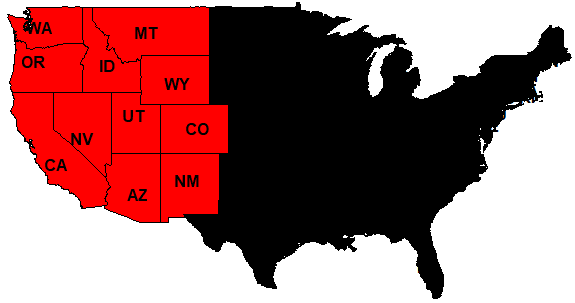
\includegraphics[width=0.8\textwidth]{WesternStatesNoTitleCropped.png}
% \caption{\label{fig:Map11States}Map of 11-state study area.} % The text after \label{} is what shows up as the caption. Inside the brackets for \label{} is just for linking figures to text and is analogous to the AuthorYear in citations. 
% \end{figure}
%%%%% End of figure with map of western US NOT next to text

% Let's plan on adjusting the figure location and decide about putting text next to figures on Friday... it's best to do that after all of the text is complete.
% For more info on floats and location specifiers, see: 
% https://en.wikibooks.org/wiki/LaTeX/Floats,_Figures_and_Captions

For the creation of the spatiotemporal daily exposure surface via machine learning, a large number of data sets will be collected as discussed below. The dependent variable will be daily 24-hour PM\textsubscript{2.5} from monitoring data.  

%We will download PM\textsubscript{2.5} data from both the  US Environmental Protection Agency (US EPA) Air Quality System (AQS) Air Data Query Tool 
We will download PM\textsubscript{2.5} data from both the US EPA AQS Air Data Query Tool 
%\citep{EPAAirData2017} and the Interagency Monitoring of Protected Visual Environments (IMPROVE) monitors that capture air quality information in 
\citep{EPAAirData2017} and the IMPROVE monitors that capture air quality information in 
more rural areas \citep{EPANPM25IMPROVE2017} for the 11-state region (Figure \ref{fig:Map11States}) including any of the following parameter codes: 88101, 88500, 88502, 81104 \citep{EPANPM25Memo2017,EPANPM25Parameters2017,EPANAllParameters2017}. In 2014, there were approximately 1600 PM\textsubscript{2.5} monitors (Figure %\ref{fig:MapLocations}
). For the 7-year study period, we anticipate approximately 1.4 million monitor-days. 
%We will use 10-fold cross-validation on a subset of this PM\textsubscript{2.5} data to train the model at monitor locations and then predict PM\textsubscript{2.5} at any location within the modeling domain. Another subset of this data will be used to quantify the accuracy of the model.
%this is stated elsewhere, so I think we don't need to state this in the data section

% %%%%% KEEP BELOW - Start Example of how to put text next to figure.
% \vspace{-6pt}
% \begin{minipage}{0.5\textwidth} % change the # on this line to adjust size of figure, as fraction of text width, also start mini page for figure
% \begin{figure}[H] % start figure float, this method seems to have fewer options for location specifier, H, t, c, and b should work
% 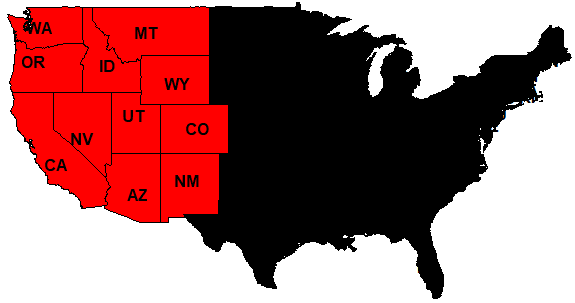
\includegraphics[width=1\textwidth]{WesternStatesNoTitleCropped.png} %
% \caption{\label{fig:Map11States}Map of 11-state study area.} % The text after \label{} is what shows up as the caption. Inside the brackets for \label{} is just for linking figures to text and is analogous to the AuthorYear in citations. 
% \end{figure} % end figure float
% \vspace{6pt}
% \end{minipage} \hfill % end mini page for figure
% \begin{minipage}{0.4\textwidth} % start mini page for text; adjust room allowed for figure have to manually set the paragraph indentations with \hspace{}
% \startsquarepar\hspace{0.25in}We will use AOD estimates from the Deep Blue retrieval algorithm for AOD from the MODIS instrument on the NASA Terra and Aqua satellites (MOD04\_L2 and MYD04\_L2) \citep{Sayer2013} and the Geostationary Operational Environmental Satellite West (GOES-West) Aerosol Smoke Product (GASP-West AOD). The MODIS product is available twice daily at a 10 km spatial resolution for cloud-free scenes and is available longer than our 2008-2014\stopsquarepar
% \end{minipage} % end mini page for text
% \vspace{-6pt}
% %%%%% KEEP ABOVE - END Example text

% \begin{figure}[ht] % [h] suggests that the figure should be "here". Other specifiers are listed at https://en.wikibooks.org/wiki/LaTeX/Floats,_Figures_and_Captions
% \centering
% 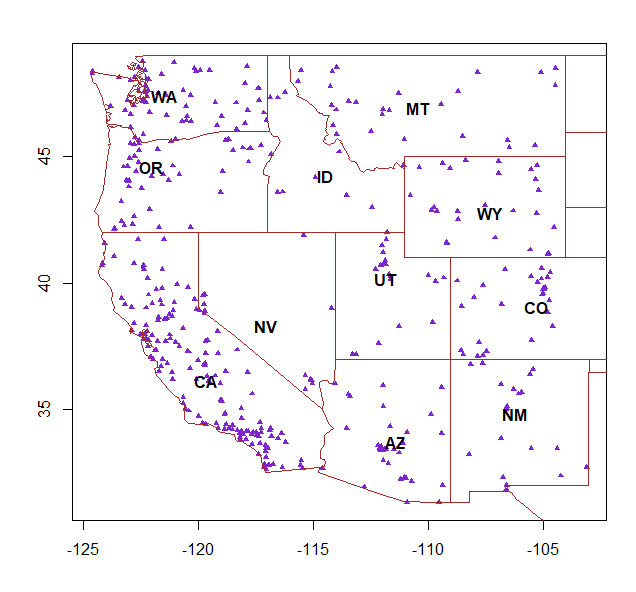
\includegraphics[width=0.8\textwidth]{m88101and88502notitlenorlabels.PNG}
% \caption{\label{fig:MapLocations}Map of 88101 and 88502 PM\textsubscript{2.5} Monitors.} % The text after \label{} is what shows up as the caption. Inside the brackets for \label{} is just for linking figures to text and is analogous to the AuthorYear in citations. 
% \end{figure}

%We will use aerosol optical depth (AOD) estimates from the Deep Blue retrieval algorithm for AOD from the MODIS instrument on the NASA Terra and Aqua satellites (MOD04\_L2 and MYD04\_L2) \citep{Sayer2013} and the Geostationary Operational Environmental Satellite West (GOES-West) Aerosol Smoke Product (GASP-West AOD). The MODIS product is available twice daily at a 10 km spatial resolution for cloud-free scenes and is available longer than our 2008-2014 
\noindent study period 
\citep{MODISMOD04L22017,MODISMYD04L22017}. The GASP product is available at a 4 km resolution at nadir with retrievals every 30 minutes during daylight hours and is available from 2006 onward 
\citep{GASPAerosolProduct2017}. Our previous work has demonstrated that the higher temporal and spatial resolution of the GASP product better predicts PM\textsubscript{2.5} compared to MODIS, but both contributed important information to our forecasting model \citep{Reid2015}. Our previous work (Table 3 from Reid et al., 2015), however, used the Dark Target retrieval algorithm rather than the Deep Blue AOD from MODIS. It is possible that the MODIS AOD from the Deep Blue algorithm will be a more informative predictor in our study area, as it has many reflective surfaces for which Deep Blue performs better than Dark Target \citep{NASADarkTarget2017}. 

% %%%%% KEEP BELOW - Start Example of how to put text next to figure.
% \begin{minipage}{0.5\textwidth} % change the # on this line to adjust size of figure, as fraction of text width, also start mini page for figure
% \begin{figure}[H] % start figure float, this method seems to have fewer options for location specifier, H, t, c, and b should work
% 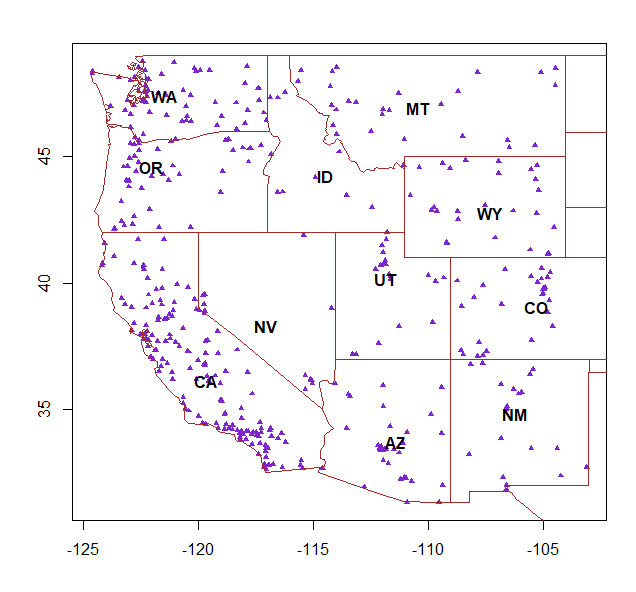
\includegraphics[width=1\textwidth]{m88101and88502notitlenorlabels.PNG} %
% \caption{\label{fig:MapLocations}Map of 88101 and 88502 PM\textsubscript{2.5} Monitors.} % The text after \label{} is what shows up as the caption. Inside the brackets for \label{} is just for linking figures to text and is analogous to the AuthorYear in citations. 
% \end{figure} % end figure float
% \vspace{6pt}
% \end{minipage} \hfill % end mini page for figure
% \begin{minipage}{0.4\textwidth} % start mini page for text; adjust room allowed for figure have to manually set the paragraph indentations with \hspace{}
% \hspace{0.25in}\startsquarepar \hspace{0.25in}AOD products use cloud filtering algorithms that often remove pixels in the center of the smoke plumes because they are assumed to be clouds due to high reflectivity \citep{kondragunta_revisions_2009}. Given that these can be in the middle of smoke plumes, often the locations most heavily impacted by smoke have missing data for a key variable, AOD. In our previous work in summer in California when rain clouds are incredibly rare, we could be confident that missing values not along the coast were not clouds. However, for this larger study region and time period, this will be a bigger challenge. We will attempt to isolate smoke plumes from true clouds using satellite imagery and smoke plume polygons from NOAA's Hazard Mapping System Fire Smoke \stopsquarepar
% \end{minipage} % end mini page for text
% \vspace{-6pt}
% %%%%% KEEP ABOVE - END Example text

\noindent Product  \citep{NOAAHazMap2017}. We will then estimate missing values within validated smoke plumes, but not within clouds, using radial basis functions as was done in our previous work \citep{Reid2015}. Radial basis functions are exact interpolation functions that will return observed AOD values where they exist but can interpolate higher values than nearby observations in missing locations, which is needed since the missing values were removed due to their high reflectivity \citep{Reid2015}.

%AOD products use cloud filtering algorithms that often remove pixels in the center of the smoke plumes because they are assumed to be clouds due to high reflectivity \citep{kondragunta_revisions_2009}. Given that these can be in the middle of smoke plumes, often the locations most heavily impacted by smoke have missing data for a key variable, AOD. In our previous work in summer in California when rain clouds are incredibly rare, we could be confident that missing values not long the coast were not clouds. However, for this larger study region and time period, this will be a bigger challenge. We will attempt to isolate smoke plumes from true clouds using satellite imagery and smoke plume polygons from NOAA's Hazard Mapping System Fire and Smoke Product \citep{NOAAHazMap2017}. We will then estimate missing values within validated smoke plumes, but not within clouds, using radial basis functions as was done in our previous work \citep{Reid2015}.



We will collect data about fire detection locations, size, and fire radiative power from the MODIS Thermal Anomalies/Fire Daily L3 Global 1km (MOD14 and MYD14), Landsat-derived burned area essential climate variable (BAECV) fire activity data, MODIS/Terra and Aqua Burned Area Monthly L3 Global 500 m SIN Grid V006 (MCD64A1), and the Visible Infrared Imaging Radiometer Suite (VIIRS) (VNP14IMGTDL\_NRT) 
\citep{Giglio2006,Hawbaker2017,MODISBurnArea,Schroeder2014}. 
Using GIS techniques, we will create daily clusters of fire points and use these to calculate: (1) the distance to the nearest fire cluster by day and (2) the sum of Fire Radiative Power (FRP) of the nearest clusters of fires by day as it is likely that smoke levels are higher closer to fires. The MODIS product spans longer than our study period (2008-2014) at daily temporal resolution and has a spatial resolution of 1 km. VIIRS was launched in 2011 and has 12 h temporal resolution with 750 m resolution. The BAECV can detect fires larger than 4 km\textsuperscript{2} and provides an estimate of the date of the fire and is available from 1984-2015. 

% \begin{figure}[ht] % [h] suggests that the figure should be "here". Other specifiers are listed at https://en.wikibooks.org/wiki/LaTeX/Floats,_Figures_and_Captions
% \centering
% \includegraphics[width=1\textwidth]{Reid2015ESTTable3.PNG}
% \caption{\label{fig:Reid2015Table3}Table 3 from \cite{Reid2015}.} % The text after \label{} is what shows up as the caption. Inside the brackets for \label{} is just for linking figures to text and is analogous to the AuthorYear in citations. 
% \end{figure}

%Classified land cover information from the Landsat-derived National Land Cover Database 2011 (NLCD 2011) 
Classified land cover information from the Landsat-derived NLCD 2011 
\citep{Homer2017} will be used to calculate estimates of the percentage of urban development (codes 22, 23, and 24), agriculture (codes 81 and 82), and vegetated area other than agricultural land (codes 21, 41, 42, 43, 52, and 71) within buffer radii of 100 m, 250 m, 500 m, and 1000 m around each monitor. The buffer distance that is most highly correlated with PM\textsubscript{2.5} will be entered into each model. NLCD 2011 has a spatial resolution of 30 m and uses circa 2011 Landsat satellite data. 

We will use snow cover data from the MODIS Snow Cover Daily L3 Global 500m Grid, Version 6 (MOD10A1 and MYD10A1) \citep{Hall2016} because snow coverage is a known contributor to wintertime PM\textsubscript{2.5} concentrations in mountain valleys \citep{Whiteman2014}. Daily MOD10A1 and MYD10A1 data are available since 2002 and have 500 m spatial resolution. 

Elevation can influence PM\textsubscript{2.5} concentrations; for example, PM\textsubscript{2.5} can accumulate in mountain valleys during persistent cold air pools 
(commonly referred to as inversions) 
during winter \citep{Whiteman2014}. We will get elevation data from the 3D Elevation Program, which has resolution of 1/3 arc-second. This resolution is approximately 10 m north/south and varies east/west with latitude \citep{USGSElevation2017}.

We will obtain meteorological data from the National Centers for Environmental Prediction (NCEP) North American Regional Reanalysis (NARR) \citep{Mesinger2006,NCEPReanalysis2005} because it includes all of the standard meteorological variables but also has planetary boundary layer height, which has proved to be an important variable for converting AOD to PM\textsubscript{2.5} \citep{liu_estimating_2005}. We will calculate 24-hour averages from 3-hourly data for temperature, relative humidity, sea level pressure, surface pressure, planetary boundary layer height, dew point temperature, precipitation, and the U and V components of wind speed. NARR has 32 km resolution and is available from 1979 onward.  

Dust storm records will be included in the machine learning algorithm because they can be a significant indicator of airborne particulate matter from sources other than fires. Dust storm records are available from 1993-2017. The spatial resolution varies, but includes either forecast zone or county  \citep{NWSstorms2017,NWSrecordhistory2017,NWSInstructions2016}.

Since traffic emissions are a well-known source of PM\textsubscript{2.5}, we will create a proxy for proximity to traffic emissions as the total distance of major roads within the buffer radii used for the land cover data. We will use the National Highways Planning Network, which includes approximately 450,000 miles of interstates, principal arterials, and rural minor arterials \citep{NHP2017}.

We will also use total PM\textsubscript{2.5} and the fire-type source-apportioned PM\textsubscript{2.5} from the Comprehensive Air Quality Model with Extensions (CAMx) \citep{CAMx2017}. See \nameref{sec:CAMxDataSources} (Section \ref{sec:CAMxDataSources}) below for further details about CAMx. 

\subsubsection{Data Sources for CAMx Modeling of Source-Attributed Air Quality Modeling}\label{sec:CAMxDataSources}

For meteorological inputs, the CAMx modeling will use archived daily 27-km Advanced Research Weather Research and Forecasting (WRF-ARW) grids available via NOAA Real-time Environmental Applications and Display sYstem (READY) servers for the entire study area and time period \citep{Wang2007,Rolph2017}. For the study years 2008-2012 and 2014, we will use fire emissions datasets prepared by the Western Regional Air Partnership (WRAP) and the National Emissions Inventory (NEI) \citep{EPANEI2017} based on aggregated source-tagged fire occurrence 
%data sources, the Fuel Characteristic Classification System (FCCS) \citep{Ottmar2007}, and Consume \citep{Prichard2009} 
data sources, the FCCS \citep{Ottmar2007}, and Consume \citep{Prichard2009}
modeling. For the study year 2013, we will prepare a fire emissions dataset using the same aggregated source-tagged fire occurrence data sources and FCCS/Consume modeling framework in the NASA-funded  Wildland Fire Emissions Information System (WFEIS) \citep{WFEIS2017} developed by Co-I's French and Billmire \citep{French2014}. Fire occurrence datasets include MODIS  (MOD14/MYD14 and MCD64A1) and  VIIRS (VNP14IMGTDL\_NRT) fire data products \citep{Giglio2006,MODISBurnArea,Schroeder2014}. %VIIRS was launched in 2011 \citep{Schroeder2014} - this is already stated above. 
For non-fire emissions during the entire study period, we will use the dataset prepared by WRAP for year 2008.

\paragraph{Statistical Analysis} [Describe statistical analysis here]

% * <melissa.maestas@colorado.edu> 2017-11-28T23:15:02.466Z:
% 
% Idea: Maybe instead of just distance to closest fire, we should follow the example of [Baek2016] and do distributed lags with concentric circles with information about fires in each concentric circle... also, instead of just distance to fire, maybe we could come up with a variable that is something like [distance*size of fire] since both are important.
% 
% ^.

\subsubsection{Spatiotemporal Surface of Total \texorpdfstring{PM\textsubscript{2.5}}{}}

In previous work \citep{Reid2015}, we used machine learning techniques to select among 10 statistical algorithms and 29 variables from globally available data sets for PM\textsubscript{2.5} for the 2008 northern California wildfires that had a CV-R\textsuperscript{2} of 0.80 using the generalized boosting method (GBM), using 13 of the 29 predictor variables \citep{Reid2015}. When we re-analyzed the data with only certain subsets of the data, we found that tree-based algorithms such as GBM and random forest could get very high predictive performance (CV-R\textsuperscript{2} values > 0.70) with different satellite measures of AOD and meteorological data (see Figure 4 ``Table 3 from Reid et al., 2015"). %shown in \nameref{MLdataSources} (Section \ref{MLdataSources}). 
We will catalyze on this method to create a similar model for a much larger spatial area (11 western states: Arizona, California, Colorado, Idaho, Montana, Nevada, New Mexico, Oregon, Utah, Washington, Wyoming) and longer time period (2008-2014). This larger area and longer time period are necessary to have the statistical power to detect associations between PM\textsubscript{2.5} from prescribed fires and health, as prescribed fires tend to occur in more rural areas and at lower concentrations.

% \begin{figure}[ht] % [h] suggests that the figure should be "here". Other specifiers are listed at https://en.wikibooks.org/wiki/LaTeX/Floats,_Figures_and_Captions
% \centering
% \includegraphics[width=1\textwidth]{Reid2015ESTTable3.PNG}
% \caption{\label{fig:Reid2015Table3}Table 3 from \cite{Reid2015}.} % The text after \label{} is what shows up as the caption. Inside the brackets for \label{} is just for linking figures to text and is analogous to the AuthorYear in citations. 
% \end{figure}

To make our daily fine spatial resolution total PM\textsubscript{2.5} model for the western US, we will use as potential predictor variables the data sets described in \nameref{MLdataSources} (Section \ref{MLdataSources}). %The outcome variable in this modeling strategy is the PM\textsubscript{2.5} values %values or value, singular?
%observed at monitoring stations throughout the western US. 
The model is trained on PM\textsubscript{2.5} values from monitoring data. 
All statistical modeling will be done in R \citep{Rproject2017} using the caret \citep{Rcaret2017} and caretEnsemble \citep{RcaretEnsemble2017} packages. We will use 10-fold cross validation to select the optimal number of variables to minimize the root mean squared error (RMSE) for a given statistical algorithm. Comparing cross validated (CV) RMSE across algorithms can yield the optimal subset of covariates for the optimal statistical model. Although we hypothesize from our previous work and that of others \citep{Reid2015,BrokampExposure2017,PandeyPredicting2013}, that a tree-based model such as GBM or Random Forest will provide the best results, ensemble learners, models that combine results from multiple algorithms, are increasingly being used and often have higher predictive performance \citep{DaviesOptimal2016}. Therefore, we will not only assess the performance of the following algorithms (generalized linear models, generalized additive models, random forest, generalized boosting models, elastic nets, multivariate adaptive regression splines, support vector machines, partial least squares, k nearest neighbors, and neural networks) that represent a diversity of statistical approaches, we will also assess if a linearized combination of these algorithms, one type of ensemble, improves predictive performance.

We will select the optimal algorithm or ensemble based on the smallest CV-RMSE, its agreement with observed data, characteristics of its residuals, and its model fit. 
We will set aside a portion of the PM\textsubscript{2.5} monitoring data as a validation data set that will not be used in any of the folds of training data in the machine learning algorithm. We will also calculate the RMSE that compares the validation data with the corresponding estimates from the optimal algorithm. The CV-RMSE of the model gives us a sense of the uncertainty in the model estimates that will then be used in the epidemiological analysis to adjust for the error in using this model to estimate exposures (see below).

\subsubsection{Attribution of \texorpdfstring{PM\textsubscript{2.5}}{} to Prescribed Fires and Wildfires}

Attributing PM\textsubscript{2.5} to prescribed fire and wildfire 
requires (1) tagging fire occurrences by fire type, (2) calculating quantity and timing of emissions from those occurrences, and (3) tracking those emissions as they disperse throughout the atmosphere.

To achieve (1), we will take advantage of existing fire occurrence datasets that have been tagged by fire type. For years 2008, 2011, and 2014, we will use datasets developed for the EPA NEI using the SmartFire v2 information system \citep{SmartFire2017,Raffuse2009}. SmartFire v2 aggregates fire occurrence data from multiple sources. Several of these sources include fire type designations, e.g., Incident Command Summary (ICS-209) reports by on-the-ground fire managers and Monitoring Trends in Burn Severity (MTBS) \citep{ICS2017,Eidenshink2007} Landsat-derived fire perimeters. For sources that do not include fire type designations (e.g., MODIS/VIIRS Active Fire and Burned Area Products), fire type is inferred based on land cover (e.g., agricultural land cover is assumed to indicate prescribed agricultural burning) and timing (i.e. fires occurring during region-specific fire seasons are assumed to be wildfire).  Under previous work, the Western Regional Air Partnership (WRAP), used similar methods to tag fire type to fire occurrence data sources for the non-NEI years 2009, 2010, and 2012. To fill out the 2008-2014 time series, we will use the same methods to tag known and inferred fire type to ICS-209, MTBS, and MODIS- and VIIRS-derived fire occurrence data sources for 2013.

To achieve (2), we will rely on existing fire emissions datasets developed via the BlueSky \citep{BlueSky2017} modeling framework for NEI (2008, 2011, 2014) and by WRAP (2009, 2010, 2012). For 2013, we will calculate emissions using the 2013 fire occurrence datasets described in (1) and the NASA-funded Wildland Fire Emissions Information System (WFEIS) \citep{WFEIS2017} developed by Co-I's French and Billmire \citep{French2014}. The WFEIS uses the same modeling framework used by both BlueSky for NEI and the Fire Emissions Tracking System (FETS) \citep{FETS2017} used by WRAP. This framework uses the 1-km Fuel Characteristic Classification System (FCCS) \citep{Ottmar2007} fuelbed map as well as the Consume consumption calculator \citep{Prichard2009}. We will use the same set of updated emissions factors used in FETS (see \cite{PMDETAIL2017}). The output of this step will be daily geospatial representation of fire emissions for 2008-2014 tagged by fire type for the entire study area.

For (3), the fire emissions data described under (2) will be formatted for input to the CAMx 6.40 gridded photochemical dispersion model \citep{CAMx2017}. WRAP previously modeled source-apportioned fire emissions using CAMx for 2008 and 2011, and so we will model years 2009-2010 and 2012-2014 in CAMx with WRAP’s consultation to ensure similar parameterization to the 2008 and 2011 runs. CAMx was the photochemical model used by WRAP primarily due to its particulate source apportionment technology (PSAT) tool, allowing the tagging and tracking of the emissions sources that contribute to downwind particulate concentrations. We will prepare PSAT to track two fire types (wildfire and prescribed fire) as well as a third category indicating non-fire. For non-fire emissions inputs, we will use the baseline 2008 non-fire emissions dataset prepared by WRAP for all modeled years, with the assumption that non-fire emissions do not vary significantly from year to year. For meteorological inputs, we will use archived daily 27-km WRF-ARW grids available via NOAA READY servers \citep{Wang2007,Rolph2017}. We will use Message Passing Interface (MPI) and Open-MultiProcessing (Open-MP) multiprocessing approaches on MTRI's computing cluster to expedite modeling runs. Outputs for this task will include daily 27-km grids of source-apportioned PM\textsubscript{2.5}. For each PM\textsubscript{2.5} source and ZIP code, we will calculate daily mean PM\textsubscript{2.5} concentration as well as the ratio of that source’s PM\textsubscript{2.5} to total PM\textsubscript{2.5}. Uncertainty in smoke modeling outputs will be assessed by comparing surface-level CAMx modeled PM\textsubscript{2.5} concentrations to PM\textsubscript{2.5} monitor data from the monitoring data described above.

\subsubsection{Measurement error}

[Consider accounting for measurement error via a nonparametric bootstrap, see \cite{Keller2017} (not sure if this applies for the paper that is just on exposure)]

\section{Performance Measures}
% 1 page
% This section must articulate the metrics and measures (both quantitative and qualitative) the team will use to determine the outcomes, results, and value of the project. The measures should, at a minimum, include those that the partner/end user/decision-making organization(s) employ to assess their decision making and services as well as those used to establish the baseline performance.
%Strategically timed calls with end users to ensure we are progressing towards products that they will use in their decision-making

%%Melissa, let's discuss the clarity of this section tomorrow.

During our project kick-off meeting, partners from state air quality and public health departments will present about their respective state-specific baseline performance measures on decision-making related to prescribed fires and wildfires. This will allow us to benchmark current decision-making processes, identify difficulties in communicating across state-level bureaucracy, and identify what information is limiting their decision-making. These states have already identified that a lack of information on health impacts associated with prescribed fires means that they are making decisions based on the assumption that the levels of PM\textsubscript{2.5} denote where health impacts occur, but that empirical evidence for historical fires could help inform or improve those decisions. 

Some of the state partners have already provided us with information on how they currently measure performance related to fire smoke. For example, the department of health in Washington measures baseline performance as the levels of PM\textsubscript{2.5} and the number of deaths, hospitalizations, and emergency department visits for respiratory and cardiovascular health endpoints on days with smoke. New Mexico is trying to allow more prescribed fires in their interagency smoke coordination and communication plan that they review annually, but they get pushback from the public with many complaints about prescribed fire planning and smoke levels. They plan to measure baseline as the number of complaint calls to the department of health and the environment department and then see if those numbers change after providing information to the public from our proposed project about associations between air pollution from prescribed fires and wildfires and respiratory and cardiovascular health. 

For our project, we will use the following measures to denote performance: (1) how much does each agency use empirical information of the health impacts of fires for their decision-making, and (2) how well do the public health and air quality managers in a given state collaborate/communicate with each other related to their decision-making related to prescribed and wildfires. We will assess this repeatedly through the project. Therefore, we will be at an ARL 3 (detailed characterization of the user decision-making process completed) by the end of the first quarter of the grant, having started at ARL 2 (decision-making activity to be enhanced by the application identified). 

In each annual meeting with the state partners, we will assess the extent to which they are using health-based information in their smoke decision-making and that the results from our investigations are influencing those decisions. We hope to be at ARL 4 by the end of year 1 of the grant, and getting to ARL 7 by the end of the project. This will be demonstrated by states proving that they are using information on the health impacts of prescribed fires in their smoke management plans and in their public health messaging during such fires. To get beyond ARL 7 we recognize will require further funding, which our group hopes to pursue during the third year of this grant such that the decision-making activity can be further enhanced with more health information. By engaging with our state-level health partners, we expect to learn more about their needs in order to contribute to a sustained decision-making process.


\section{Discussion}

[text from NASA grant as starting point]

This work directly addresses NASA's desire to ``discover and demonstrate innovative and practical uses of Earth observations'' by using several Earth observations, including several MODIS, Landsat, and VIIRS products, to spatiotemporally estimate ground-level PM\textsubscript{2.5} concentrations and combine this information with Medicare data so that we may better understand the health impacts of smoke from both prescribed fires and wildfires in the western US. Using satellite data and other Earth observations allows us to estimate air quality in locations without air quality monitors. \textbf{Our results will be used by both state air quality managers in updating their smoke management plans and state health departments for targeted communication related to health-protective measures during prescribed fires and wildfires.} All of this work is directly applicable to NASA's Health and Air Quality Application area's interest in the use of Earth observations in air quality management and public health. By working with the NASA Earth Science Division (ESD)/Applied Sciences socioeconomic consortium to coordinate our research and results, the work proposed could be of interest to other NASA Applied Sciences activities.

Our work falls under NASA's Second Strategic Goal in the 2014 Strategic Plan to ``advance understanding of Earth and develop technologies to improve the quality of life on our home planet'' within the realm of Objective 2.2 to ``advance knowledge of Earth as a system to meet the challenges of environmental change, and to improve life on our planet.'' Wildfires are a significant source of air pollution that impacts the health of human populations, particularly in the western US. Prescribed fires are one way to decrease high-intensity catastrophic fires, but without empirical knowledge of the health impacts of prescribed fires compared to wildfires, it is difficult for all stakeholders to come to consensus about the use of prescribed fires. 
Our work will inform how the western US decides to manage its forests to minimize health harms from ecologically necessary fires on the landscape. 

The relevance of our work to decision-makers in both air quality and public health is apparent by the \textbf{incredible outpouring of support we have received from WESTAR and EPHTN as well as their state partners}. This is exemplified in the letters of support that are part of our proposal submission. We had more letters of support than we were allowed to submit with this application, thus EPHTN and WESTAR leaders offered to compile one letter of support from all of their state partners who were interested. The WESTAR letter of support implies that all state air quality managers provide their support, even though they are not enumerated. We also received individual letters of support from some air quality managers before they knew about the combined WESTAR letter. We have included the letter from Colorado as an example of these letters that we also received from New Mexico and Washington. 

\section{Anticipated Results and Improvements}
% 1 page
% This section describes the expected results and improvements to the decision-making activity from the application and integration of Earth observations. This section should articulate the expected improvement(s) over the "baseline" performance of the decision-making activity.

%[paragraph re-write below]Many state smoke management programs were put into place to assist states with implementing measures to reduce regional haze. Smoke management and difficulties communicating across agencies is often seen as an impediment to more prescribed fires in the US \citep{SneeuwjagtOpportunities2013}. In addition to this, decisions about when and where to set prescribed burns is done based on air quality, but without information related to the health impacts associated with smoke from wildfires and prescribed fires; these decisions are being done without complete information. Thus the baseline performance of these decisions is based on a presumption that if the air quality impacts of the prescribed fire are low, then the health impacts will also be low. According to our state partner collaborators, no information on health associated with changes in air quality is known but just assumed because no one has yet done an analysis such as the one presented here. 
Many state smoke management programs were put into place to assist states with implementing measures to reduce regional haze. Smoke management and difficulties communicating across agencies are often seen as impediments to more prescribed fires in the US \citep{SneeuwjagtOpportunities2013}. In addition to this, decisions about when and where to set prescribed burns are made based on air quality, but without information related to the health impacts associated with smoke from wildfires and prescribed fires. Since these decisions are being made without complete information, the baseline performance of these decisions is based on a presumption that if the air quality impacts of the prescribed fire are low, then the health impacts will also be low. According to our state partner collaborators, no information on health impacts associated with smoke from prescribed fires is known but just assumed because no one has yet done an analysis such as the one presented here. 

The state partners are enthusiastic about this project because it will provide them with information to influence their smoke management planning and public health messaging. For example, if we find that there are significant health impacts of prescribed fires at levels below the national ambient air quality standard, this could cause smoke management plans to modify the use of prescribed fires to have lower impacts on air quality. On the other hand, if we find that there are no significant health impacts from prescribed fires, or that they begin to occur at higher levels of PM\textsubscript{2.5}, then smoke management plans may be modified to allow more burning. Similarly in regards to public health decision-making, more targeted messaging for how to protect oneself during fires could be employed for different types of fires if there are indeed differential health impacts. Currently, messaging is the same regardless of fire type \citep{EPA2016}. %change this last refernce to see this for more information on recommendations for public health messaging for wildfires smoke. 
% not sure what to put here. A few ideas:
% \citep{Olsen2017} - about public acceptance of various fire types - https://doi.org/10.1071/WF16034
% https://www.epa.gov/air-research/wildfire-smoke-and-health-risk-communication-workshop-and-report ... featured talk by Olsen
% https://www.epa.gov/air-research/wildland-fire-research-health-effects-research

Our project can provide information that will help at the state air program/state health department interface. In years 2 and 3, we have budgeted funds for members of the research team (a to-be-determined subset of Drs. Reid, Maestas, and French) to travel to conferences/meetings attended by the state air quality managers and by the state public health departments to update them on progress in the grant and disseminate results that can influence their decision-making. 

Given that \textbf{the decision-making we aim to influence is done through combined intersections of air quality managers and public health professionals, our partnering with both groups is essential.} We have received enthusiastic support from all state air quality managers in our region who are part of WESTAR and all state public health departments who are part of EPHTN. By having support from both agencies in most states in our region (not all western states are part of EPHTN), we hope that we will have the most success in those states (Arizona, California, Colorado, New Mexico, Oregon, Utah, and Washington) for using empirical evidence of the health impacts of smoke from prescribed fires and wildfires. Through our collaboration with air quality managers in the other states (Idaho, Montana, Nevada, and Wyoming), we hope to make connections to their public health departments and provide them with data and results from our analyses. We recognize that this endeavor will be a long-term process that may not occur for all states within the three years of this project. As we learn more about the decision-making related to prescribed fires and the challenges each state has with effective communication, we will be able to identify ways forward through further projects and grants. 

\section{Transition \& Sustainability Plan}

% 1 page
% 	This section should identify major issues (e.g., management, organization, technical) affecting the adoption and sustained use of the application. Accounting for these items, this section should articulate the proposed transition plan, including specific activities within the timeframe of the project to enable the end-user organization(s) to adopt the enhancements in their decision support activity (or new decision support activity). The section should describe activities (e.g., training, workshops) to support and enable the sustained use of the Earth observations and enhanced decision making.
% webinars with end-users to explain data and their interpretation and use
Research translation to decision-making will be an on-going activity during our three-year project, and will proceed based on consultation with our state-level partners. The information that is co-developed between the research team and state decision-making partners will be the most impactful. We will have regular meetings with the research team and collaborators to ensure that we all understand the goals of the project and to update our decision-makers about our progress. 

We will begin with a project kick-off in Boulder, Colorado at the beginning of the grant in summer 2018. We have budgeted funds for travel for many of our participants and will additionally have web-cast capabilities through Earth Lab at CU Boulder to involve those who cannot attend in person. Each spring, the researchers will travel to a conference attended by the WESTAR state partners, such as the WESTAR business meeting, and one attended by the EPHTN states, such as the Environmental Public Health Tracking Workshop. To ensure effective adoption of the information, it is essential for us to start the project on the same page of what the intended methods, outcomes, and uses of the data are by all parties. 

Throughout the tenure of the grant, we will be meeting in person (at conferences the decision-makers attend) annually and by phone/internet biannually, with the state air quality managers and public health professionals. These meetings will be ways to update our partners on our progress and hear from them about ways that we could better meet their informational needs related to decision making for prescribed fires and wildfires. 

In the last year of the grant, we will survey our state partners about how they intend to use the information we have provided, whether they will continue to use this information, and what information they still need for continued use of the information in prescribed fire decision making. Sustained development and transition of the products will depend on the needs identified through this process. Since data on health impacts from prescribed fire has not been available before this project, we anticipate our project to be just the beginning of a long-term exchange of how valuable science-based information can be made useful for decision-making. 

\section{Acknowledgements}

WESTAR, EPTHN (unless they are on the author's list)

PM\textsubscript{2.5} data from the Uintah Basin were provided by Seth Lyman at Utah State University. [look over full documentation file to determine full list of acknowledgements]

%\section{Bibliography styles}

%There are various bibliography styles available. You can select the style of your choice in the preamble of this document. These styles are Elsevier styles based on standard styles like Harvard and Vancouver. Please use Bib\TeX\ to generate your bibliography and include DOIs whenever available.

%Here are two sample references: \cite{Feynman1963118,Dirac1953888}.

\section*{References}

%\bibliography{mybibfile}
\bibliography{ReidGroupReferences}

%\section{PM2.5 Surface Paper Notes}

\subsection{Papers published in Atmospheric Environment used as style example}

Need to go through these papers
\begin{itemize}
\item \cite{BrokampExposure2017} (partially done, done through abstract)
\end{itemize}



\subsection{Notes on Papers}

Put in \cite{BrokampExposure2017}
 % COMMENT THIS WHEN PAPER IS MOSTLY DONE
\section{Ideas, To Do, Resources, etc}

Consider using the work of Westerling et al for a comprehensive fire history (up through 2012) \url{http://science.sciencemag.org/content/313/5789/940}, \url{http://www.pnas.org/content/108/32/13165}, \url{http://rstb.royalsocietypublishing.org/content/371/1696/20150178} \cite{westerling_increasing_2016,WesterlingCorrection2016} Also look into the fire histories referenced in Westerling \cite{westerling_increasing_2016,WesterlingCorrection2016}: \url{http://fam.nwcg.gov/fam-web/weatherfirecd/fire_files.htm} and \url{http://fam.nwcg.gov/fam-web/kcfast/mnmenu.htm} See also \url{http://www.nifc.gov}

Look at \cite{kollanus_effects_2016} again for references for PM2.5 paper, especially the introduction. Consider using NAAPS in our study. 

Idea: look at ambulance calls and PM2.5, similar to what \cite{salimi_ambient_2016} did in Australia.

US National Atlas \url{http://nationalmap.gov/small_scale/atlasftp.html}

Thought: Using DigitalGlobe for fire data compared to NASA: would have higher spatial resolution, but not consistently viewing all areas (no cost to CU people) 
% Sentinal only goes back a couple of years

%Look

Papers/resources to look into: \url{https://daac.ornl.gov/cgi-bin/dsviewer.pl?ds_id=1293}

\url{https://www.fs.fed.us/psw/publications/4451/psw_2009_4451-001.pdf}

\url{https://labcit.ligo.caltech.edu/~ethrane/Resources/UNIX/}

\url{https://community.tableau.com/thread/141548}

According to \cite{liu_particulate_2016}, GEOS-Chem ``can be classified according to emission source'', that implies that we could tag the emissions as wildfire vs prescribed fire vs urban. Would there be any advantages of this model over CAMx?

could analyze data with NAAQS and WHO PM2.5 standards

projection/datum info: \url{https://gis.stackexchange.com/questions/664/whats-the-difference-between-a-projection-and-a-datum}
\url{http://resources.esri.com/help/9.3/arcgisengine/dotnet/89b720a5-7339-44b0-8b58-0f5bf2843393.htm}
\url{http://grindgis.com/blog/wgs84-vs-nad83}

Monitoring Trends in Burn Severity (MTBS) MTBS, 2016: Data Access: Fire Level Geospatial Data. USDA Forest Service/U.S. Geological Survey, accessed 8 October 2016, https://mtbs.gov/direct-download. 
Eidenshink, J., B. Schwind, K. Brewer, Z.-L. Zhu, B. Quayle, and S. Howard, 2007: A project for monitoring trends in burn severity. Fire Ecol., 3, 3–21, https://doi.org/10.4996/fireecology.0301003. 

Idea: Maybe instead of just distance to closest fire, we should follow the example of [Baek2016] and do distributed lags with concentric circles with information about fires in each concentric circle... also, instead of just distance to fire, maybe we could come up with a variable that is something like [distance*size of fire] since both are important.

Fire stats/records: \url{https://www.nifc.gov/fireInfo/fireInfo_statistics.html}

\section{PM2.5 Surface Paper Notes}

Discussion of trends in anthro PM2.5: \cite{ridley_causes_2018}

\subsection{Papers published in Atmospheric Environment - use as style example}

Need to go through these papers
\begin{itemize}
\item \cite{BrokampExposure2017} (partially done, done through intro)
\item \cite{Sampson2013}
\item \cite{Anyenda2016}
\item \cite{Torvela2014}
\item \cite{Whiteman2014}
\end{itemize}

Put in \cite{BrokampExposure2017,larsen_impacts_2017}

\section{Papers to cite/discuss in Introduction and/or Discussion}

\cite{westerling_increasing_2016,WesterlingCorrection2016}

try to find English version \url{http://80.24.165.149/webproduccion/PDFs/15CAP03.PDF}

\subsection{Notes on Papers}

See \cite{Fusco2016} for statistics about wildfires in western US, e.g., \% started by humans, number of fires, etc.

\section{Fire attribution paper}

include \cite{long_aligning_2018} - does a good job of summarizing the debate about more vs less prescribed burns

include \cite{westerling_increasing_2016,WesterlingCorrection2016} and \cite{abatzoglou_impact_2016}

See \cite{Kaulfus2017} for an alternative method of attributing PM2.5 to wildfire smoke (instead of CAMx)

\end{document}